
\subsection{Results}

On the post-test check,
for each stimuli set participants achieved at least 91\% accuracy
in correctly identifying that the base and correct response option
belonged to the same biological category,
and at least 68\% accuracy in correctly identifying that
the base and the foil option \emph{did not} belong to the same category
(binomial tests by participant, N = 59, p's < .0075;
minimum accuracy required for p < .01 is 40/59, or 67.8\%).
Post test scores for each stimulus set are included
in Appendix~\ref{appendix:exp1_posttest}.
Therefore, data from all stimulus sets
were included in the analyses.


I analysed the data using linear or logistic mixed models,
with random intercepts for each participant and each stimulus set,
and random coefficients for the effect of condition for each participant
(see Chapter 2).
Participants selected the foil species
on 4\% of trials in the control condition,
and 40\% of trials in the conflict condition;
$e^{\beta}$ = 209.1, CI = [3.6; 12169.2],
z = 2.577, p = .0100).
Therefore, perceptual similarity had a robust effect on their responses,
leading them to generalise the property to a foil species
belonging to a different biological group,
rather than to the base species,
considerably more often when the base and foil looked alike.


It is worthwhile assessing the pattern of individual differences in this effect.
Figure~\ref{fig:exp1_acc} shows the number of foil responses
each participant gave, by condition.
Forty nine participants were more likely to select the foil under conflict,
eight never selected it, and two showed the reverse effect, selecting the foil
less often under conflict.
Therefore, it appears that the effect of visual similarity
holds across almost all of the participants.

\begin{figure}[ht]
  \centering
  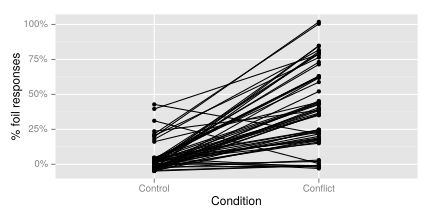
\includegraphics[width=\figurewidth]{imgs/exp1_acc.pdf}
  \caption{
    Proportion of foil responses given by each participant, per condition, in Experiment 1.
    \label{fig:exp1_acc} }
\end{figure}

The time taken to begin moving the mouse cursor (initiation time; IT),
and to select a response option (response time; RT)
both had positively-skewed distributions,
and so were log-transformed before analysis.
For correct responses,
there were no significant differences in IT between conditions,
taking 976 msec under conflict (SD = 1,000)
and 881 msec in the control condition (SD = 772; t = 0.104, p > .9).
However, RT was significantly slower
for conflict trials (2,668 msec, SD = 1,564)
than control trials (2,112 msec, SD = 1,279;
$e^{\beta}$ = 122.9\%, CI = [114.2\%; 132.3\%], t(58.5) = 5.553, p < .0001).

\begin{table}
  \centering
  \begin{tabular}{lrrrr}
    \toprule
    Condition & Response time & Initiation time & Reversals\\
    \midrule
    Control   & 2,112 (1,279) & 881 (772)       & 19\%\\
    Conflict  & 2,668 (1,564) & 976 (1,000)     & 43\%\\
    \midrule
    p         & < .0001      & > 0.9           & < .0001\\
    \bottomrule
  \end{tabular}
  \caption[Descriptive statistics for correct responses, Experiment 1.]{
    Summary statistics for correct responses in each condition.
    Standard deviations are shown in parentheses.
    Correct responses under conflict took significantly longer,
    and were more likely to be classed as \emph{reversals}.
    There was no difference in movement initiation times.
    }
\end{table}



Maximum Deviation (MD) % was also significantly higher
% for conflict trials (0.71, SD = 0.79)
% than for control trials (0.35, SD = 0.57;
% $\beta$ = 0.37, CI = [0.22; 0.51],
% t(54.0) = 5.128, p < .0001).
% However, MD
was bimodally distributed
(Bimodality Coefficient = .667;
Hartigan's D = 0.025, N = 453, p = .0058),
with trajectories either going directly to the selected response,
or moving towards one response, and changing direction mid-flight
(see Appendix~\ref{appendix:reversals}).
Trajectories were therefore classed as either \emph{direct} or \emph{reversals},
as described in Chapter 2.
When selecting the correct species,
participants were significantly more likely
to initially move towards the foil option
on conflict trials (37.7\%)
than on control trials (15.9\%;
$e^{\beta}$ = 4.8, CI = [2.5, 9.3], z = 4.699, p < .0001).

As discussed in Chapter 2,
there were therefore four kinds of mouse trajectories
observed in this experiment:
direct movements to the correct option (\emph{Direct Correct}),
initial movements towards the foil, which changed direction
to the correct option (\emph{Reversal Correct}),
initial movements towards the correct option, which changed direction
to the foil (\emph{Reversal Foil}),
and direct movements  to the foil (\emph{Direct Foil}).
Table~\ref{tbl:exp1_trajectories} shows how common
each trajectory type was in both conditions,
and indicates substantial increases in both incorrect responses
and reversal correct trials,
and a decrease in direct correct trials, under conflict.

\begin{table}
  \centering
  \begin{tabular}{lrrrr}
    \toprule
             & Direct Correct & Reversal Correct & Reversal Foil & Direct Foil\\
    \midrule
    Control  & 77.5\%         & 18.7\%           & 1.7\%         & 2.1\%\\
    Conflict & 34.4\%         & 25.8\%           & 8.2\%         & 31.6\%\\
    \bottomrule
  \end{tabular}
  \caption[Kinds of trajectory in Experiment 1.]{
    The four different possible kinds of cursor trajectory,
    broken down by condition.
    \label{tbl:exp1_trajectories}}
\end{table}

These different kinds of trial can be better understood
in terms of their \emph{transition probabilities} (see Chapter 2).
At the beginning of a trial, participants either move towards the correct option,
with probability $\alpha$, or towards the foil, with probability $1 - \alpha$.
After initial movement towards the correct option, they can either
select this option, with probability $\beta$, or the foil, with probability $1 - \beta$.
Finally, after moving towards the foil, participants can either
change direction and give the correct response,with probability $\gamma$,
or persevere and select the foil option, with probability $1 - \gamma$.
Figure~\ref{fig:exp1_transitions} shows
a schematic of these probabilities.
Table~\ref{tab:exp1_transitions_table}
show each of them across both conditions.
Again, these probabilities were compared using logistic mixed models,
with random intercepts for each stimulus set,
and random intercepts and slopes for each participant.

Participants were significantly more likely to
initially move towards the correct response in the control condition
(79\% of trials)
than the conflict condition (43\%;
regression $e^{\beta}$ = 7.3, CI = [4.7; 11.3], z = 8.773, p < .0001).
After doing so, they were also more likely to then select the correct response
in the control condition (98\%) than the conflict condition
(81\%; regression $e^{\beta}$ = 25.9, CI = [6.6, 101.2],
z = 3.078, p = .0021).\footnotemark
Finally, on trials where they did initially move towards the foil,
participants were more likely to eventually select the correct species
in the control condition (90\%)
than in the conflict condition (45\%;
regression $e^{\beta}$ = 26.6, CI = [7.0; 101.2], z = 4.815, p < .0001).

\begin{figure}[ht]
  \begin{floatrow}
    \ffigbox[.5\textwidth]{%
    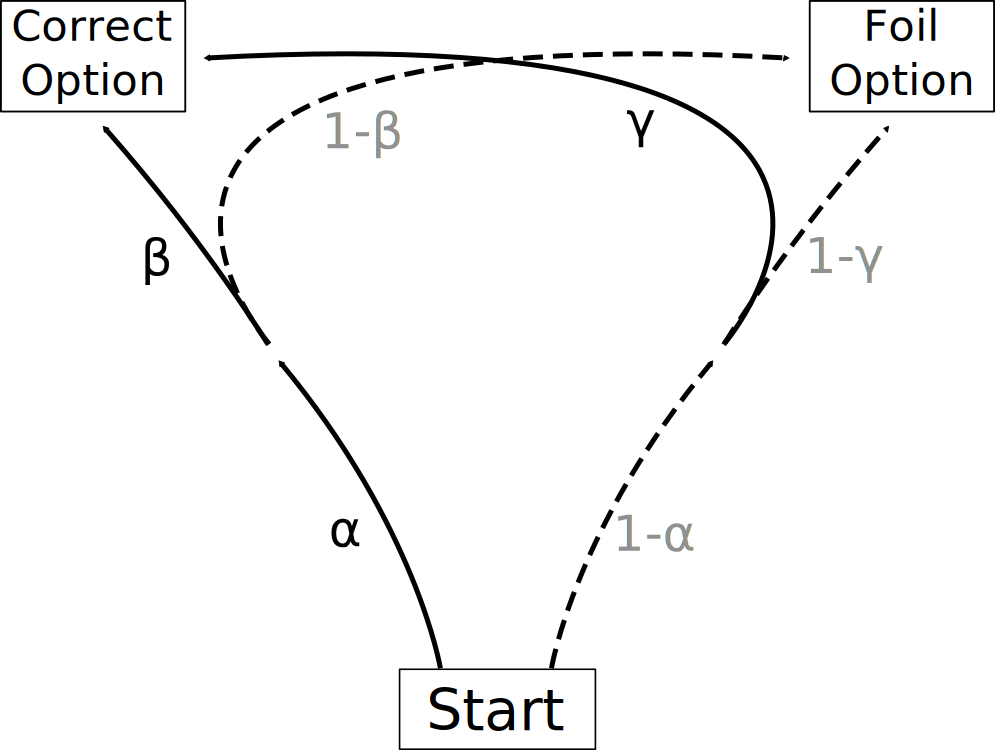
\includegraphics[width=.5\textwidth]{../2.Methods/imgs/transitions.pdf}
    }{%
      \caption{
        The possible cursor transitions that can occur during a trial.
        \label{fig:exp1_transitions}
    }
    }
    \capbtabbox{%
      \centering
      \begin{tabular}{lrr}
        \toprule
        Parameter & Control & Conflict  \\
        \midrule
        $\alpha$  & 79\%    & 43\%$^{**}$\\
        $\beta$   & 98\%    & 81\%$^{**}$\\
        $\gamma$  & 90\%    & 45\%$^{**}$\\
        \bottomrule
        \multicolumn{3}{l}{
          \emph{Note}: $^{**}p < .01$.
        }
      \end{tabular}
      %% \begin{tabular}{cc} \hline
      %%   Author & Title \\ \hline
      %%   Knuth & The \TeX book \      Lamport & \LaTeX \\ \hline
      %% \end{tabular}
    }{%
      \caption{
        Transition probabilities for Experiment~1.
        \label{tab:exp1_transitions_table}
      }%
    }
  \end{floatrow}
\end{figure}


\footnotetext{
  As the value for the control condition was close to 1,
  regression parameters here would normally approach $\infty$,
  and the model would be unidentifiable,
  a phenomena known as \emph{perfect separation}
  \citep{Albert1984}.
  I therefore used penalised-likelihood estimation
  to impose an uninformative prior distribution \citep{Zorn2005}
  on the regression parameters, effectively reflecting a belief
  that when observed probabilities are close to 0 and 1,
  the true probabilities are likely to be higher, or lower, respectively.
  In this, and all future cases of perfect separation, I impose
  a Gaussian prior on the regression weights,
  with mean 0 and standard deviation 3.
}

Finally, if the processes drawing participants
towards selecting the foil on conflict trials operate early in reasoning,
we would expect movements towards this option to be initiated earlier
than those towards the correct species.
I found this to be the case,
with initial movements towards the foil initiated
after 687 msec on average (SD = 599),
and those towards the correct species initiated
after 1,182 msec (SD = 1,119).
Fitting a mixed model with random intercepts
for each participant and each stimulus set,
this difference was found to be significant;
$e^{\beta}$ = 130\%, CI = [120\%, 150\%], t(204.6) = 4.042, p < .001).


\subsubsection{Time course}

In order to investigate \emph{when} participants' mouse cursor movements
were drawn towards each response option,
I examined the position of the cursor over the first 4 seconds of each trial.
As participants largely moved discretely to one or other response,
these positions were not normally distributed,
and so I coded the location of the cursor
according to whether or not it was on the foil species' side of the screen.
By doing so, it is possible to identify at what points in time
participants' mouse movements are guided by perceptual similarity,
which drives participants towards selecting the foil species on conflict trials
(see Chapter 2).

\begin{figure}[tp]
  \centering
  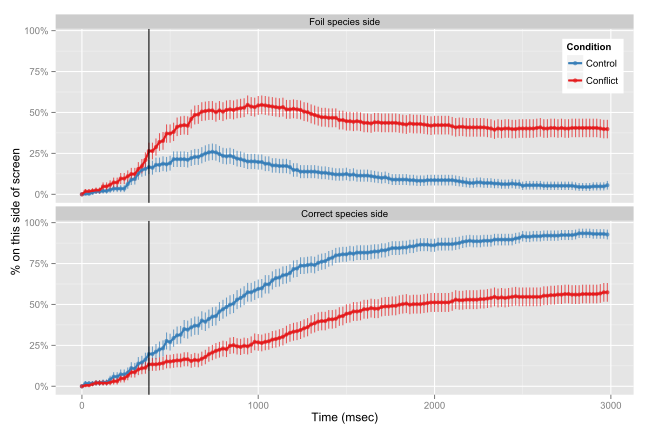
\includegraphics[width=.8\textwidth]{imgs/exp1_condition_timecourse.pdf}
  \caption[Time course, separately for each response option, in Experiment 1.]{
    Time course of attraction towards each response option.
    Vertical lines show the points from which
    the difference between the two conditions is
    statistically significant (p < .05).
    Error bars show 95\% confidence intervals.
    \label{fig:exp1_condition_timecourse}
  }
\end{figure}

\begin{figure}[bp]
  \centering
  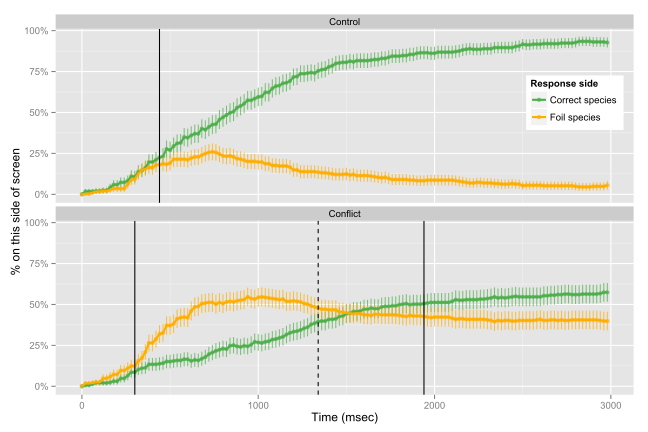
\includegraphics[width=.8\textwidth]{imgs/exp1_side_timecourse.pdf}
  \caption[Time course, separately for each condition, in Experiment 1.]{
    Time course of attraction towards each response option.
    Solid lines show the points from which one response
    is significantly more likely to be moved towards than the other (p < .05),
    while dashed lines for the points from which
    these differences are no longer significant.
    Error bars show 95\% confidence intervals.
    \label{fig:exp1_side_timecourse}
  }
\end{figure}

Figure~\ref{fig:exp1_condition_timecourse} shows the proportion of trials
on the side of the screen corresponding to each response option.
I fitted two series of logistic mixed models,
predicting the probability of being on the foil's side of the screen,
and one the probability of being on the correct species' side of the screen.
Each series consisted of a set of models,
one fitted to every 20 msec time window,
with condition as a predictor, 
and random intercepts for each participant, and each base species.
I used these series of models to find the divergence points:
the time from which participants were significantly more likely to move towards
the foil species in conflict trials than control trials,
and the time from which they were significantly more likely to move towards
the correct species in control trials than conflict trials.
In both cases, these significant differences between the conditions
emerged from 380 msec onwards.


Figure~\ref{fig:exp1_side_timecourse} shows
the same data, but with separate lines for each side of the screen,
and separate facets for each condition.
In the control condition, participants were significantly more likely
to move towards the correct option than the foil
from 440 msec onwards.
In the conflict condition, however, we see the interaction of
the two competing cues.
Participants were significantly more likely to move towards
the foil option from 300 msec.
This preference for the foil persisted until 1,340 msec,
at which stage both response options were equally popular.
From 1,940 msec, finally, participants were more likely to
move towards the correct option than the foil,
as the initial attraction towards the foil option
has been largely inhibited.
In other words, participants were
initially drawn towards the foil species on conflict trials,
but were later drawn towards the correct species instead.

\FloatBarrier


